% Template for ICIP-2026 paper; to be used with:
%          spconf.sty  - ICASSP/ICIP LaTeX style file, and
%          IEEEbib.bst - IEEE bibliography style file.
% --------------------------------------------------------------------------
\documentclass{article}
\usepackage{spconf,amsmath,graphicx}
% Chinese support (XeLaTeX)
\usepackage{fontspec}
\usepackage{xeCJK}
% Prefer Noto CJK fonts; fallback to WenQuanYi if unavailable.
\IfFontExistsTF{Noto Serif CJK SC}{
  \setCJKmainfont{Noto Serif CJK SC}
}{
  \IfFontExistsTF{Noto Sans CJK SC}{
    \setCJKmainfont{Noto Sans CJK SC}
  }{
    \IfFontExistsTF{WenQuanYi Zen Hei}{
      \setCJKmainfont{WenQuanYi Zen Hei}
    }{
      \IfFontExistsTF{AR PL UMing CN}{
        \setCJKmainfont{AR PL UMing CN}
      }{
        % Last resort: let XeTeX try system default (may still warn).
        \setCJKmainfont{SimSun}
      }
    }
  }
}
\IfFontExistsTF{WenQuanYi Zen Hei Mono}{\setCJKmonofont{WenQuanYi Zen Hei Mono}}{}
% Better Chinese line breaking
\XeTeXlinebreaklocale "zh"
\XeTeXlinebreakskip = 0pt plus 1pt

% Example definitions.
% --------------------
\def\x{{\mathbf x}}
\def\L{{\cal L}}

% Title.
% ------
\title{CoReGate:基于反事实贡献分解与可靠性门控的稳健多模态情感分析}
%
% Single address.
% ---------------
\name{Author(s) Name(s)\thanks{Thanks to XYZ agency for funding.}}
\address{Author Affiliation(s)}
%
% For example:
% ------------
%\address{School\\
%	Department\\
%	Address}
%
% Two addresses (uncomment and modify for two-address case).
% ----------------------------------------------------------
%\twoauthors
%  {A. Author-one, B. Author-two\sthanks{Thanks to XYZ agency for funding.}}
%	{School A-B\\
%	Department A-B\\
%	Address A-B}
%  {C. Author-three, D. Author-four\sthanks{The fourth author performed the work
%	while at ...}}
%	{School C-D\\
%	Department C-D\\
%	Address C-D}
%
\begin{document}
%\ninept
%
\maketitle
%
\begin{abstract}

\end{abstract}
%
\begin{keywords}
Multimodal sentiment analysis, counterfactual contribution, reliability gating, robust fusion
\end{keywords}
%
\section{INTRODUCTION}
\label{sec:intro}

多模态情感分析(Multimodal Sentiment Analysis, MSA)旨在综合文本、音频与视觉等线索,对用户表达的情感强度或极性进行预测,是人机交互与多模态理解中的基础任务之一~\cite{zhu2024review}。尽管融合能够引入互补信息,但在真实场景中非语言模态往往更易受采集条件、背景噪声、遮挡与缺失等因素影响,并可能与文本语义发生冲突(例如讽刺或反语),从而使“直接融合”既可能带来收益,也可能放大误差并导致性能不稳定~\cite{williams2018dnn,wang2022cross}。

\begin{figure}[t]
  \centering
  \includegraphics[width=0.98\linewidth]{figures/fig1}
  \caption{Motivation of robust fusion. Naive fusion may amplify errors when audio/vision are noisy, missing, or conflicting with text.}
  \label{fig:intro_motivation}
\end{figure}

现有研究主要从融合算子、表示学习与鲁棒性建模等角度推进 MSA。早期/中间/晚期融合工作系统比较了特征拼接、表征融合与决策加权等策略~\cite{williams2018dnn,williams2018recognizing};张量融合通过显式高阶外积建模跨模态交互,但会引入高维开销与潜在过拟合风险~\cite{zadeh2017tensor,liu2018efficient};序列建模方法进一步刻画跨时间的交互与记忆更新~\cite{zadeh2018memory,zadeh2018multimodal}。与此同时,表示学习路线尝试缓解模态差异与冗余(例如共享/私有子空间分解)~\cite{tsai2019learning,hazarika2020misa},或借助自监督/多任务信号强化模态特异信息~\cite{yu2021learning}。近年来,文本主导的跨模态增强与文本引导融合得到关注,通过将非语言线索注入文本表征以提升未对齐场景下的效果~\cite{wang2022cross,wang2023tetfn};此外也有工作从对比去噪或不完整模态学习角度提升鲁棒性~\cite{wang2025contrastive,jiang2025boosting}。

尽管上述方法有效提升了平均性能,但在“强文本、弱且不稳定的非语言模态”这一现实设置下,一个核心困难仍未被充分解决:当音频/视觉噪声、缺失或与文本冲突时,融合模型往往缺少对非语言信息\emph{何时有益、何时有害}的可控机制,因而容易将不可靠证据注入预测并放大误差~\cite{williams2018dnn,zadeh2017tensor,zadeh2018memory,wang2022cross,wang2023tetfn,wang2025contrastive,jiang2025boosting}。因此,我们希望构建一种以文本为主干、对非语言信息进行可解释且可控的增量注入方式,使模型在退化场景下能够自然退化并保持稳健(见 Fig.~\ref{fig:intro_motivation})。

为此,我们提出 CoReGate(Counterfactual Reliability-Gated Fusion),将非语言模态建模为对文本预测的\emph{增量修正}:分别学习文本分支、文本+音频分支与文本+视觉分支的预测,并用“加入某一模态前后预测的差分”来显式刻画该模态带来的边际修正;随后由样本级可靠性门控根据表征线索与模态质量统计,选择性注入这些修正,从而在音频/视觉退化或与文本冲突时抑制不可靠信息并自然退化到更稳健的文本主干。

我们的主要贡献总结如下:
\begin{itemize}
  \item 提出一种基于反事实贡献分解与可靠性门控的稳健融合框架,将非语言模态显式建模为对文本预测的增量修正,实现可控注入与自然退化。
  \item 在 CMU-MOSI 与 CMU-MOSEI 上的实验表明,所提方法在标准评测与缺失模态压力测试下均具有稳定的性能与鲁棒性优势。
\end{itemize}

\section{PROPOSED METHOD}
\label{sec:method}

本节提出一种基于反事实贡献分解(counterfactual contribution decomposition)与可靠性门控(reliability gating)的稳健融合框架。我们以文本预测为主干,并将音频与视觉视作对文本的\emph{增量证据}:模型输出三个分支预测(\(T\)、\(TA\)、\(TV\)),由此构造边际贡献,再通过样本级门控选择性注入贡献项,从而在噪声或冲突模态存在时仍保持稳健。整体流程示意见 Fig.~\ref{fig:framework}。

\begin{figure*}[t]
  \centering
  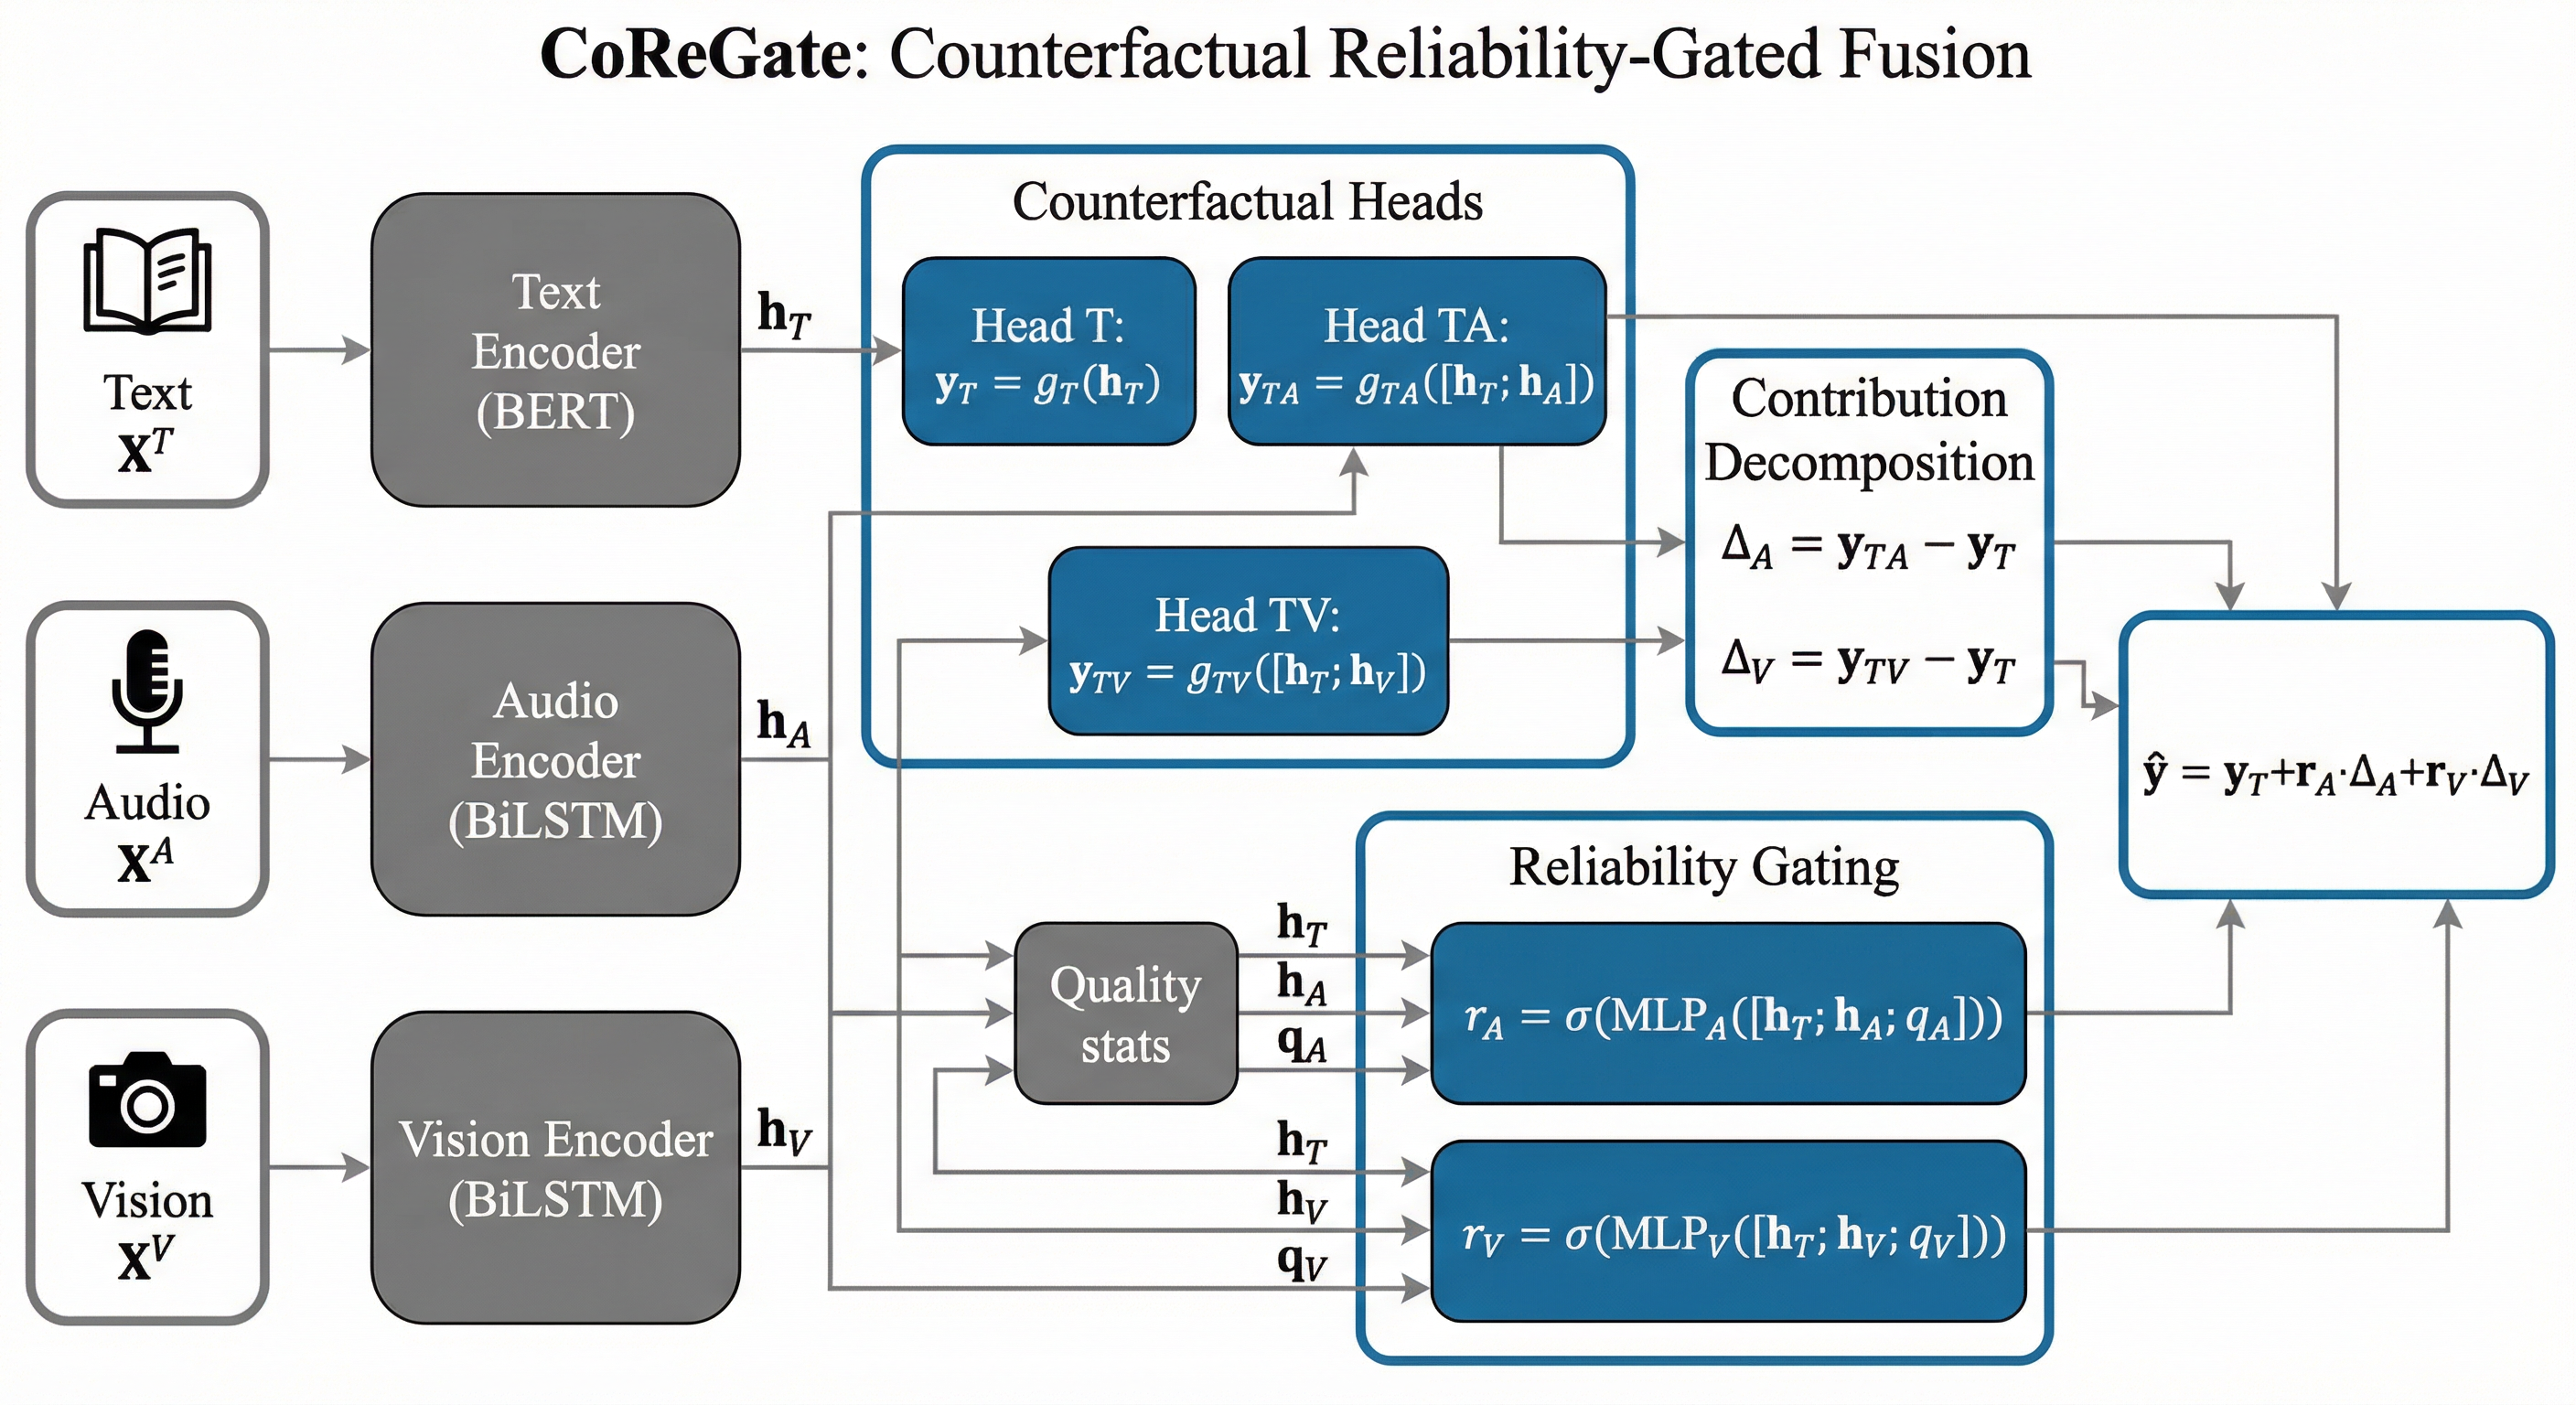
\includegraphics[width=0.98\textwidth]{figures/fig2.png}
  \caption{Overview of CoReGate. Text is treated as a backbone predictor. Audio/vision provide marginal increments (\(\Delta_A,\Delta_V\)) estimated by counterfactual heads and injected by sample-wise reliability gates (\(r_A,r_V\)).}
  \label{fig:framework}
\end{figure*}

如 Fig.~\ref{fig:framework} 所示,我们先分别编码三模态得到 \(\mathbf{h}_T,\mathbf{h}_A,\mathbf{h}_V\),并训练三个分支预测器得到 \(y_T,y_{TA},y_{TV}\)。由此计算边际贡献 \(\Delta_A,\Delta_V\),再由门控网络结合表征线索与质量统计 \((\mathbf{q}_A,\mathbf{q}_V)\) 预测可靠性系数 \(r_A,r_V\),最终在输出层对增量进行选择性注入,以在模态退化时抑制不可靠增量并自然退化到文本主干。

\subsection{Problem Formulation}
\label{ssec:form}
给定三模态输入 \((\mathbf{X}^{(\mathrm{T})},\mathbf{X}^{(\mathrm{A})},\mathbf{X}^{(\mathrm{V})})\),目标是预测连续情感强度 \(y\)(回归标量)。为避免与“转置”记号混淆,我们使用 \(\mathrm{T}/\mathrm{A}/\mathrm{V}\) 作为模态索引。我们以一个共享表征空间中的多分支预测器建模不同模态子集的输出。具体地,令 \(\mathbf{h}_m = E_m(\mathbf{X}^{(m)})\) 为模态 \(m\in\{\mathrm{T},\mathrm{A},\mathrm{V}\}\) 的句级表征,并对任意模态子集 \(S\subseteq\{\mathrm{T},\mathrm{A},\mathrm{V}\}\) 定义融合与回归映射,得到分支预测
\begin{equation}
y_S = g_S\!\left(f_S\big(\{\mathbf{h}_m\}_{m\in S}\big)\right),\quad S\in\{\mathrm{T},\mathrm{TA},\mathrm{TV}\}.
\end{equation}
在下文中,我们以 \(y_T\) 作为文本主干输出,其余分支用于构造可控且便于分析的增量贡献。

\subsection{Encoders and Representations}
\label{ssec:enc}
我们将文本、音频与视觉分别表示为序列输入,其中音频与视觉允许与文本\emph{未对齐},并通过有效长度或掩码处理补零填充的时间步。文本编码器采用预训练语言模型提取句级表征(取 \texttt{[CLS]} 对应的隐向量作为 \(\mathbf{h}_T\))。对音频与视觉,我们使用轻量时序编码器对帧级特征进行上下文建模,得到序列隐状态后再聚合为句级表示 \(\mathbf{h}_A,\mathbf{h}_V\)。聚合阶段采用文本引导的注意力池化(以文本表征为查询,从未对齐的音频/视觉序列中选择与语义相关的时间片);当注意力不可用时,可退化为基于掩码的均值池化。上述 \(\mathbf{h}_T,\mathbf{h}_A,\mathbf{h}_V\) 将用于三分支预测与后续的可靠性门控。

\subsection{Counterfactual Contribution Decomposition}
\label{ssec:cf}

现有融合方法多依赖隐式注意力或表示对齐来平衡模态,缺少可操作、可量化的“模态贡献”定义;在仅有总体情感标签监督的条件下,模型也难以稳定学习何时应信任或抑制某模态。我们将“模态贡献”定义为\textbf{在固定其它模态条件下,加入该模态导致预测变化的差分量},从而赋予贡献明确的反事实语义,并可由多分支预测直接估计。

具体地,我们以文本为主干、将音频与视觉视为可选修正信号。设 \(y_T\) 为仅文本预测,\(y_{TA}\)、\(y_{TV}\) 分别为文本+音频、文本+视觉预测(回归任务下均为标量)。定义边际贡献为
\begin{equation}
\begin{aligned}
\Delta_A &= y_{TA}-y_T, \\
\Delta_V &= y_{TV}-y_T.
\end{aligned}
\end{equation}
直观地,\(\Delta_A\) 与 \(\Delta_V\) 分别度量音频/视觉对文本预测的净修正。这种分解将“融合增益”拆解为可计算的差分项:在方法层面,我们不再直接在特征层给出难以解释的注意力权重,而是学习“是否注入\emph{增量证据}”的门控(见下节),从而提升训练稳定性与鲁棒性。

\subsection{Reliability-Gated Fusion}
\label{ssec:gate}

在真实数据中,音频或视觉常受采集条件影响而出现噪声、缺失或与文本语义冲突;若将贡献项一律注入,不可靠模态会将预测系统性带偏。为此,我们为每个样本学习门控系数 \(r_A, r_V\in[0,1]\),以“该贡献是否可信”为准则选择性注入,最终预测写为
\begin{equation}
\hat{y} = y_T + r_A\Delta_A + r_V\Delta_V.
\end{equation}
当某模态不可靠时,对应门控趋近于 0,使预测退化为更可靠的文本主干;当非语言模态提供互补信息时,门控允许其贡献注入以修正输出。为让门控与“可靠性”语义对齐,我们将门控网络建立在\textbf{表征线索}与\textbf{模态质量统计}两类信息之上。令 \(\mathbf{h}_S\) 为分支 \(S\) 的融合表示(例如 \(f_S(\cdot)\) 的池化输出),我们构造门控输入向量
\begin{equation}
\begin{aligned}
\mathbf{z}_A &= \big[\mathbf{h}_T;\mathbf{h}_A;\mathbf{q}_A \big], \\
\mathbf{z}_V &= \big[\mathbf{h}_T;\mathbf{h}_V;\mathbf{q}_V \big],
\end{aligned}
\end{equation}
并以小型 MLP 预测门控系数:
\begin{equation}
\begin{aligned}
r_A &= \sigma(\mathrm{MLP}_A(\mathbf{z}_A)), \\
r_V &= \sigma(\mathrm{MLP}_V(\mathbf{z}_V)).
\end{aligned}
\end{equation}
其中 \(\sigma(\cdot)\) 为 Sigmoid。这里 \(\mathbf{h}_T\) 为文本表征,\(\mathbf{h}_A,\mathbf{h}_V\) 为与文本相关的音频/视觉上下文表征;\(\mathbf{q}_A,\mathbf{q}_V\) 为低维的样本级模态质量统计,用于为门控提供可靠性线索(例如缺失程度、能量强弱与稳定性等)。

\noindent\textbf{Why gating contributions (not features).}
与直接在融合特征上学习权重不同,我们对\textbf{贡献差分}施加门控,使门控更接近“是否相信该模态提供的\emph{增量证据}”。同时,\((r_A,r_V)\) 与 \((\Delta_A,\Delta_V)\) 可逐样本输出,便于对模型的模态依赖与失败模式进行诊断分析。

\subsection{Training Objective}
\label{ssec:loss}

主任务采用 MAE(L1)回归损失。为稳定各分支学习并避免某些分支退化(例如 \(TA/TV\) 学不到有效增量,导致 \(\Delta_A,\Delta_V\) 近似噪声),我们在对最终预测 \(\hat{y}\) 施加主监督的同时,对三个分支输出 \(y_T,y_{TA},y_{TV}\) 施加辅助监督,引入分支损失权重 \(\lambda\ge0\),总损失为
\begin{equation}
\mathcal{L} = \mathcal{L}_{\hat{y}} + \lambda\left(\mathcal{L}_T + \mathcal{L}_{TA} + \mathcal{L}_{TV}\right),
\end{equation}
其中 \(\mathcal{L}_{\hat{y}}\) 对最终 \(\hat{y}\) 监督,\(\mathcal{L}_T, \mathcal{L}_{TA}, \mathcal{L}_{TV}\) 分别对 \(y_T, y_{TA}, y_{TV}\) 监督。该设计保证了贡献项 \(\Delta_A,\Delta_V\) 的可学习性:若缺少对 \(TA/TV\) 的监督,差分量可能退化为噪声,从而削弱门控的有效性。

为保持可复现性,我们在补充材料中提供完整的训练设置与配置文件。

\section{EXPERIMENTAL RESULTS}
\label{sec:exp}

\subsection{Dataset and Metrics}
\label{ssec:dataset}

实验在 CMU-MOSEI 上进行情感回归;采用数据集标准划分,评价指标包括 MAE(越低越好)、相关系数 Corr(越高越好)以及离散化后的 Acc7 等,与现有 MMSA 工作一致。

\subsection{Implementation Details}
\label{ssec:impl}

模型在统一训练框架下实现,并遵循公开基线的训练流程与评测协议。我们在验证集上选择超参数,并采用早停策略防止过拟合;其余训练细节与配置将随代码公开,以保证可复现性。

\subsection{Evaluation of Our Method}
\label{ssec:main}

表~\ref{tab:main} 给出 MOSI 与 MOSEI 上主结果,评价指标包括 MAE、Corr、Acc7、Acc2(Has0/Non0)、F1(Has0/Non0)。我们在统一训练与评测协议下复现各方法,并据此进行横向比较。

\begin{table*}[t]
  \centering
\caption{CMU-MOSI 与 CMU-MOSEI 主结果。Acc2/F1 格式为 Has0/Non0(\%)。}
  \label{tab:main}
  \small
  \begin{tabular}{l|ccccc|ccccc}
    \hline
    & \multicolumn{5}{c|}{\textbf{CMU-MOSI}} & \multicolumn{5}{c}{\textbf{CMU-MOSEI}} \\
    \hline
    Models & MAE$\downarrow$ & Corr$\uparrow$ & Acc7$\uparrow$ & Acc2$\uparrow$ & F1$\uparrow$ & MAE$\downarrow$ & Corr$\uparrow$ & Acc7$\uparrow$ & Acc2$\uparrow$ & F1$\uparrow$ \\
    \hline
    EF-LSTM~\cite{williams2018recognizing} & 0.956 & 0.658 & 32.5 & 78.1/79.3 & 78.2/79.4 & 0.593 & 0.689 & 50.0 & 78.2/81.7 & 78.7/81.7 \\
    LF-DNN~\cite{williams2018dnn} & 0.992 & 0.650 & 33.2 & 76.5/77.7 & 76.6/77.9 & 0.557 & 0.728 & 53.1 & 83.6/83.7 & 83.3/83.1 \\
    TFN~\cite{zadeh2017tensor} & 0.988 & 0.640 & 35.6 & 75.1/76.1 & 75.1/76.2 & 0.565 & 0.725 & 52.7 & 80.4/83.4 & 80.9/83.4 \\
    LMF~\cite{liu2018efficient} & 0.981 & 0.637 & 36.0 & 75.4/76.2 & 75.4/76.3 & 0.562 & 0.739 & 51.5 & 81.8/83.9 & 82.1/83.8 \\
    MFN~\cite{zadeh2018memory} & 0.938 & 0.669 & 35.9 & 77.0/78.9 & 77.6/78.9 & 0.568 & 0.726 & 50.7 & 82.2/84.0 & 82.3/83.8 \\
    MFM~\cite{tsai2019learning} & 0.899 & 0.673 & 37.8 & 78.9/80.2 & 78.8/80.1 & 0.573 & 0.727 & 51.0 & 81.7/83.6 & 82.1/83.6 \\
    Graph-MFN~\cite{zadeh2018multimodal} & 0.886 & 0.693 & 37.6 & 79.6/81.0 & 79.4/80.8 & 0.562 & 0.725 & 52.1 & 83.3/83.4 & 83.1/82.8 \\
    MISA~\cite{hazarika2020misa} & 0.805 & 0.765 & 40.2 & 81.6/83.2 & 81.6/83.3 & 0.547 & 0.759 & 51.9 & 82.8/84.9 & 83.0/84.8 \\
    Self-MM~\cite{yu2021learning} & 0.726 & 0.784 & 48.0 & 82.5/84.5 & 82.5/84.5 & 0.539 & 0.765 & 52.8 & 74.8/82.0 & 76.0/82.3 \\
    TETFN~\cite{wang2023tetfn} & 0.731 & 0.790 & 45.2 & 80.9/82.8 & 80.9/82.8 & 0.546 & 0.762 & 53.9 & 80.6/85.1 & 81.1/85.1 \\
    CENET~\cite{wang2022cross} & 0.739 & 0.789 & 43.6 & 82.1/83.8 & 82.0/83.9 & 0.529 & 0.775 & 54.2 & 82.4/85.8 & 82.7/85.6 \\
    MECAM~\cite{wang2025contrastive} & 0.715 & 0.782 & 46.6 & 84.4/85.8 & 84.3/85.8 & 0.547 & 0.748 & 52.3 & 83.7/85.2 & 81.6/84.8 \\
    \textbf{Ours} & \textbf{0.716} & \textbf{0.794} & \textbf{46.9} & 82.8/84.9 & 82.7/84.8 & \textbf{0.529} & \textbf{0.775} & \textbf{54.6} & 82.0/86.5 & 82.5/86.4 \\
    \hline
  \end{tabular}
\end{table*}

\subsection{Robustness under Missing Modalities}
\label{ssec:robust}

为验证可靠性门控在退化输入下的作用,我们在测试阶段构造模态缺失设置:将音频置零(missing-A)、将视觉置零(missing-V),以及二者同时置零(missing-A+V)。在同一训练权重下,我们进一步比较门控开启(Gating ON)与强制关闭(Gating OFF,即令 \(r_A=r_V=1\))的差异。图~\ref{fig:robust_missing} 给出在 MOSI 与 MOSEI 上的 MAE 对比。

\begin{figure}[t]
  \centering
  \includegraphics[width=0.98\linewidth]{figures/fig3_missing_robustness.pdf}
  \caption{Robustness under missing modalities. We evaluate the same trained checkpoint while masking A/V at test time. Reliability gating consistently reduces MAE compared with forcing gates to 1 (Gating OFF), especially when the visual modality is missing.}
  \label{fig:robust_missing}
\end{figure}

可以看到,门控在缺失场景下带来一致且显著的鲁棒性收益。在 MOSEI 上,关闭门控会使 MAE 在三种缺失设置下均恶化约 \(+0.025\sim+0.026\)(同时 Corr 与 Acc7 也下降);在 MOSI 上,门控同样带来稳定收益,尤其在 missing-V 时 MAE 恶化达到 \(+0.021\)。该结果支持我们的核心动机:门控作用于\emph{增量修正}可在模态缺失/退化时抑制不可靠注入,使模型更自然地退化到可靠的文本主干或剩余模态。

\subsection{Ablation and Discussion}
\label{ssec:abl}

表~\ref{tab:ablation} 汇总了消融结果。我们围绕三类关键设计进行对比:\textbf{(i) 可靠性门控}(w/o gating:将 \(r_A=r_V=1\))、\textbf{(ii) 反事实分解融合形式}(t-only:仅使用文本分支 \(y_T\);a-only/v-only:仅使用单一非语言模态分支输出)、以及 \textbf{(iii) 分支辅助监督}(w/o branch sup:去除对 \(\{y_T,y_{TA},y_{TV}\}\) 的辅助损失)。

\begin{table}[t]
  \centering
  \caption{Ablation results on CMU-MOSI and CMU-MOSEI. Acc7 is reported in \%.}
  \label{tab:ablation}
  \small
  \setlength{\tabcolsep}{5pt}

  \begin{tabular}{l|ccc}
    \hline
    \multicolumn{4}{c}{\textbf{CMU-MOSI}} \\
    \hline
    Setting & MAE$\downarrow$ & Corr$\uparrow$ & Acc7$\uparrow$ \\
    \hline
    Full (CoReGate) & \textbf{0.7159} & 0.7944 & \textbf{46.94} \\
    w/o gating & 0.7211 & 0.7932 & 45.34 \\
    t-only (\(y=y_T\)) & 0.7370 & 0.7903 & 45.19 \\
    a-only (\(y=y_A\)) & 0.9342 & 0.7019 & 33.38 \\
    v-only (\(y=y_V\)) & 1.4750 & 0.1375 & 15.16 \\
    w/o branch sup & 0.7405 & 0.7903 & 44.75 \\
    \hline
  \end{tabular}

  \vspace{2mm}

  \begin{tabular}{l|ccc}
    \hline
    \multicolumn{4}{c}{\textbf{CMU-MOSEI}} \\
    \hline
    Setting & MAE$\downarrow$ & Corr$\uparrow$ & Acc7$\uparrow$ \\
    \hline
    Full (CoReGate) & 0.5286 & 0.7746 & \textbf{54.56} \\
    w/o gating & 0.5275 & \textbf{0.7771} & 54.37 \\
    t-only (\(y=y_T\)) & 0.5422 & 0.7665 & 53.21 \\
    a-only (\(y=y_A\)) & 0.5989 & 0.7129 & 48.92 \\
    v-only (\(y=y_V\)) & 0.6477 & 0.6484 & 47.97 \\
    w/o branch sup & 0.5348 & 0.7755 & 53.90 \\
    \hline
  \end{tabular}
\end{table}

从表~\ref{tab:ablation} 可得到三点结论。首先,单模态基线显示文本是最可靠的主导模态:t-only 显著优于 a-only 与 v-only(尤其在 MOSI 上 v-only 几乎失效),从而支持“以文本为主干、以 A/V 为增量修正”的建模选择。其次,去除分支辅助监督会带来明显的性能下降(尤其在 MOSI 上),表明对反事实分支(\(T/TA/TV\))的监督有助于稳定学习可用的边际贡献,从而提升最终融合效果。最后,虽然在标准测试集上门控收益在不同数据集/随机性下可能较为细微,但在模态缺失压力测试中其收益非常显著(见图~\ref{fig:robust_missing}),进一步验证了门控设计的鲁棒性动机。

此外,门控 \((r_A,r_V)\) 与贡献 \((\Delta_A,\Delta_V)\) 可逐样本输出,便于对模型何时依赖或抑制非语言模态进行诊断分析。

本方法的优势在于将"模态贡献"从隐式权重转化为可计算的反事实差分,便于在文中形成可验证的论证;局限在于门控目前仍通过主任务监督间接学习,未引入显式模态质量标签,未来可结合压力测试与更强对齐监督进一步改进。

\section{CONCLUSION}
\label{sec:conc}

本文提出基于反事实贡献分解与可靠性门控的多模态情感回归方法:通过多分支预测显式定义音频与视觉对文本预测的边际贡献,并用样本级门控选择性注入,在模态质量不一致时保持稳健预测。在 CMU-MOSEI 上,所提方法在 MAE 与 Corr 上优于 CENET 等基线。后续将补充更系统的消融与鲁棒性实验,并完善英文全文。

% References
\bibliographystyle{IEEEbib}
\bibliography{strings,refs}

\end{document}
